\chapter{Measurement of Directional Characteristics III}\label{ax:directional_3}
This appendix serves as a protocol to a series of measurements conducted between the 10\textsuperscript{th} and 12\textsuperscript{th} of May  2018 in the large anechoic chamber (B4-111) at the acoustic lab of Aalborg University at Fredrik Bajers Vej 7.\\
The goal of these measurements is investigating the behaviour of a loudspeaker array consisting of three of the loudspeakers that have been featured in \autoref{ax:directional_1} and \ref{ax:directional_2}.

\section*{Measuring Equipment and Materials}
The following measuring equipment was used:
\begin{itemize}[noitemsep]
\item Microphone \gls{bandk} 4144
\begin{itemize}[noitemsep]
\item AAU-number: 06552
\item Serial number: 297090
\end{itemize}
\item Preamplifier GRAS 26AK
\begin{itemize}[noitemsep]
\item AAU-number: 56526
\item Serial number: 32810
\end{itemize}
\item Power supply \gls{bandk} 2636
\begin{itemize}
\item AAU-number: 08022
\item Serial number: 
\end{itemize}
\item Calibrator \gls{bandk}\ 4231
\begin{itemize}[noitemsep]
\item AAU-number: 33691
\item Serial number: 2115338
\end{itemize}
\item 2 pcs. Power Amplifier Pioneer A-616
\begin{itemize}[noitemsep]
\item AAU-number: 08249, 08699
\item Serial number: HJ9404841S, JG9405804S
\end{itemize}
\item Sound card RME Fireface UCX
\begin{itemize}[noitemsep]
\item AAU-number: 108230
\item Serial number: 23811948
\end{itemize}
\item Turntable: Outline ET 250-3D
\begin{itemize}
\item Serial number: REIB0012
\end{itemize}
\item MATLAB r2017b on OSX 10.11.6
\item 3 pcs. Loudspeaker SEAS 33 F-WKA
\end{itemize}

The following material was used:
\begin{itemize}[noitemsep]
%\item \SI{1/2}{\inch} to \SI{1}{\inch} preamp adapter
\item Microphone clip
\item Microphone stand
\item LEMU cable
\item \gls{bandk} cable
\item XLR cables
\item Ethernet cable
\item miscellanious adapters
\item 3 pcs. Loudspeaker cabinet, plywood, outside dimensions: (400x400x400)\SI{}{\milli\meter}, wall~thickness:~\SI{20}{\milli\meter}, equipped with \citep{seas33}
\item Speaker mount for turntable
\begin{itemize}[noitemsep]
\item Steel mounting contraption, see REFERENCE TO HARDWARE CHAPTER
\item 3 speaker legs, \SI{40}{\milli\meter} box section, top: aluminium, {\(\varnothing\)~:~\SI{34.8}{\milli\meter}}, height: \SI{1}{\meter}
\item Circular \gls{mdf} cutout, thickness: \SI{12}{\milli\meter}, {\(\varnothing\)~:~\SI{800}{\milli\meter}}
\item \gls{mdf} cutout, thickness: \SI{20}{\milli\meter}, surface: approx. (300x600)\SI{}{\milli\meter}, bolt pattern drilled according to the bottom side of the ET 250-3D turntable
\item \gls{mdf} cutout for counterweight mounting, thickness: \SI{12}{\milli\meter}, surface : (400x400)\SI{}{\milli\meter}
\item triangular cutout (isosceles), thickness: \SI{12}{\milli\meter}, approximate outside dimensions (base width x height): (970x600)\SI{}{\milli\meter}
\item 2 Electrovoice S-200 speakers as counterweight
\item Ratchet strap
\item 4 bolts M8x80, associated washers
\item 6 bolts M8x30, associated washers
\item 8 sinkhead bolts M8x40, associated nuts and washers
\item miscellaneous woodscrews

\end{itemize}
\end{itemize}



\section*{Setup}
When setting up the speaker array according to dimensions that have been decided upon in \autoref{sec:opt_result}, a substential effort was undertaken to insure a secure stance. The turntable was mounted to one of the platform grids used in the anechoic chamber by screwing bolts through a \gls{mdf}-plate and the grid into the threads on the underside of the turntable. A round \gls{mdf} plate was mounted using the boltpattern on the upside of the turntable. Fixed to the round plate a custom made steel contraption (\autoref{fig:speakerstand}) was bolted, which itself held the legs of the speakers in place. while allowing some adjustability. In a height of approx \SI{1}{\meter} above the turntable the three speaker cabinets were mounted to the legs. On top of the speaker a triangular \gls{mdf} cutout was employed to enhance rigidity. A picture of the array is given in \autoref{fig:05_11_setup}.

\begin{figure}[h]\label{fig:05_11_setup}
	\centering
    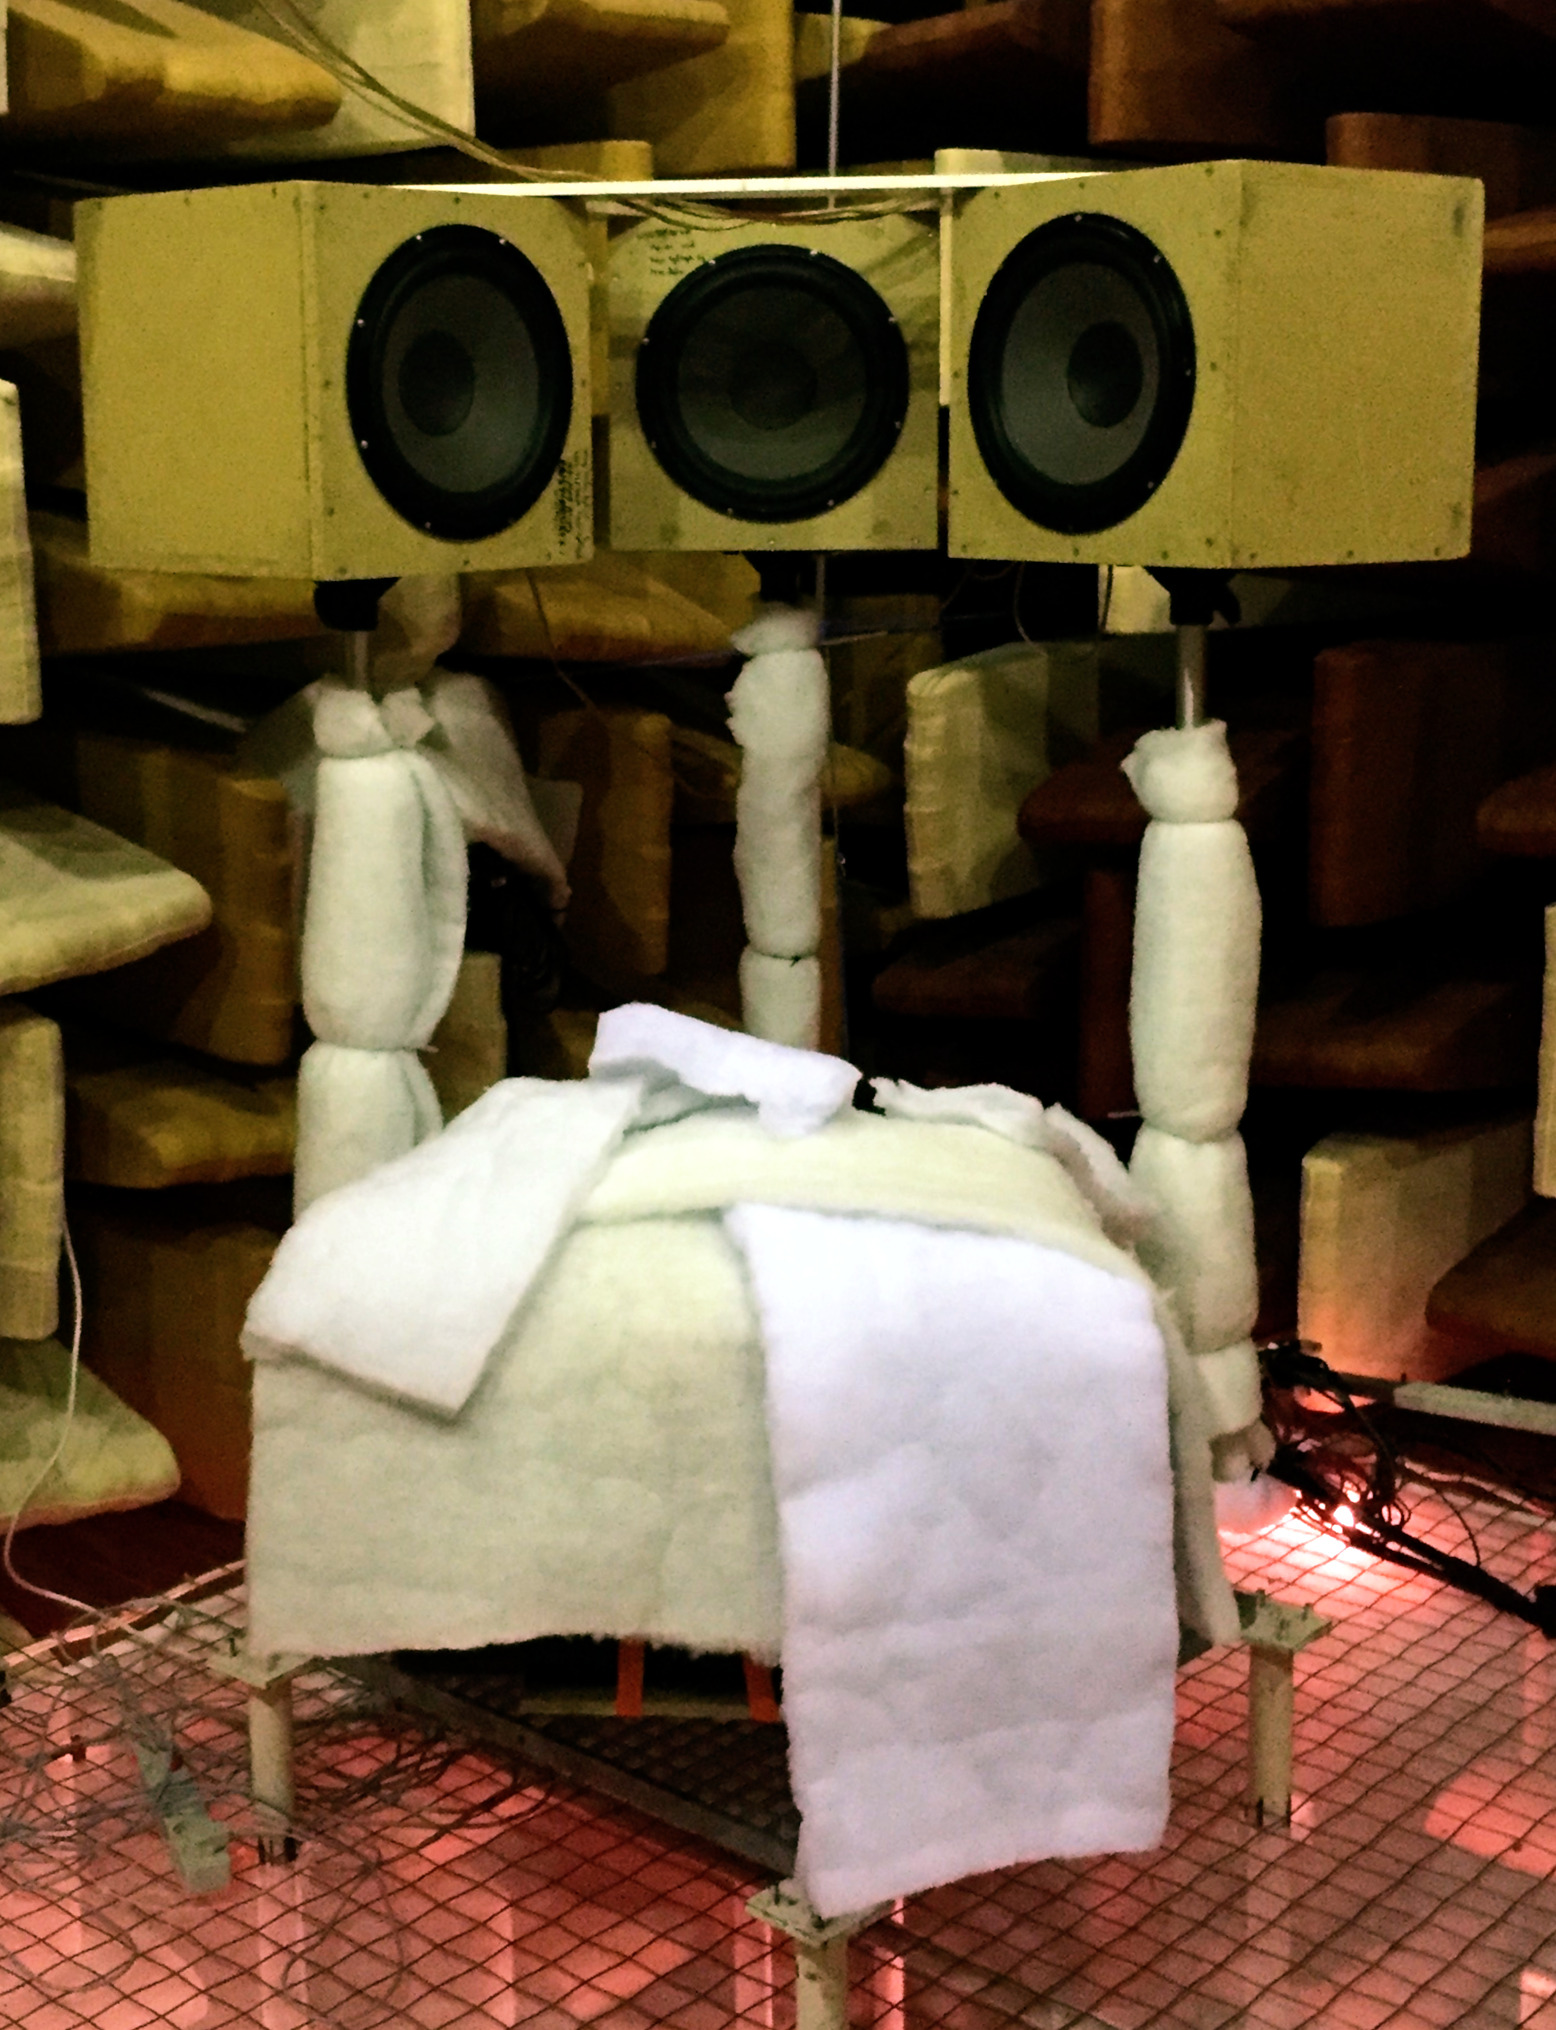
\includegraphics[width=0.5\textwidth]{05_11_setup.jpg}
    \caption{Speaker array setup on the turntable in the anechoic chamber.}
\end{figure}

The height of the centers of the speaker cabinet above the grid turned out to be \SI{1.37}{\meter}. The microphone was set up in the same height. The horizontal distancedistance between the array center and the microphone was \SI{4.92}{\meter}.
The input and the output gain of the \gls{bandk} 2636 microphone power supply were both set to \SI{+10}{\decibel}. The input gain on the Fireface UCX was set to \SI{0}{\decibel}. On the playback side, the power amplifiers had a fixed voltage gain of \SI{+10}{\decibel} and the \texttt{playgain}-parameter in the measurement routine was set to \SI{-10}{\decibel}. The playback signals were normed so that the absolute of the biggest amplitude in on of the filtered sweeps (see \autoref{sec:filter_design} is a digital value of 1.